\documentclass[11pt]{article}

% Other package to deal with references
\usepackage{nameref}

% FONTS
\usepackage[charter]{mathdesign}
\renewcommand{\sfdefault}{phv}
\usepackage[utf8]{inputenc}
\usepackage[english]{babel} % Language

\usepackage{amsmath} % Math
\usepackage{graphicx}   % Figures
\usepackage{subcaption}	
\usepackage[final]{pdfpages} % To include pdfs
\usepackage{float}
\usepackage{paralist}
\usepackage{natbib}
\usepackage{array}
\usepackage{rotating}
\usepackage{lineno}   % For line numbering
\usepackage{setspace} % For line spacing
\usepackage{xcolor}

%\usepackage{fourier}
\usepackage{microtype}
% Geometry - margins etc.
\usepackage[hscale=0.725, vscale=0.75, includehead=false, includefoot=false, marginparsep=-1.25cm]{geometry}

\usepackage[textsize=footnotesize, backgroundcolor=orange!50, bordercolor=white]{todonotes}
\usepackage{soul} % Highlighting

% SPECIFIC COMMANDS FOR THE DOCUMENT -------------------------------
\newcommand{\articletitle}[0]{} % Title of the manuscript
\newcommand{\authorlist}[0]{} % List of authors
\newcommand{\msid}[0]{\# 59535 (previous ID)} % Manuscript ID
\newcommand{\thejournal}[0]{The American Naturalist}
\newcommand{\thejournalshort}[0]{AmNat}
%-------------------------------------------------------------------

%%% HELPER CODE FOR DEALING WITH EXTERNAL REFERENCES
%---------------
\usepackage{xr-hyper}
\makeatletter
\newcommand*{\addFileDependency}[1]{% argument=file name and extension
  \typeout{(#1)}
  \@addtofilelist{#1}
  \IfFileExists{#1}{}{\typeout{No file #1.}}
}
\makeatother
 
\newcommand*{\myexternaldocument}[1]{%
    \externaldocument{#1}%
    \addFileDependency{#1.tex}%
    \addFileDependency{#1.aux}%
}

%%% END HELPER CODE ------------------------------------
\myexternaldocument{main} %% add link to the maintext file of your revised manuscript in the file list (new file, from another project). 

%% COLORS
\definecolor{darkblue}{rgb}{0,0,0.6}
\definecolor{darkred}{rgb}{0.6,0,0}
\definecolor{lgray}{gray}{0.95}
\definecolor{llgray}{gray}{0.925}
\definecolor{dgray}{gray}{0.15}
\definecolor{darkgreen}{rgb}{0.0, 0.42, 0.24} % FD I added this because it was not defined but used for Hildegard's comments
\definecolor{purple}{rgb}{0.75,0.,0.75}
\definecolor{change}{rgb}{0.5,0.,0.6}


% HEADERS & FOOTERS
\usepackage{lastpage}
 \usepackage{fancyhdr}
 \setlength{\headheight}{16pt} % Change head height otherwise warning
 \pagestyle{fancy}
 \fancyhead{}
 \fancyfoot{}
 \fancyhead[L]{\textcolor{dgray}{\textsc{\small Reply to reviewers -- Revision of manuscript \msid{}
 } }}
 \fancyhead[R]{}
 \fancyfoot[C] {\thepage{}}


% REFEREES TEXT
\definecolor{colreferee}{RGB}{0,30,50}
\definecolor{colchange}{RGB}{150, 0, 200}
\newenvironment{referee}{\vspace{0.cm} \sffamily \color{colreferee} \begin{quotation} }{\end{quotation} \vspace{0.cm}}

% NUMBER THE COMMENTS
% and add label to be able to refer to a specific comment
\newcommand{\lmarginpar}[1]{\reversemarginpar\marginpar{\textcolor{colreferee}{\textbf{\textsf{[#1]}}}}}
\newcommand{\addnb}[1]{\refstepcounter{numcom}\lmarginpar{\arabic{numcom}}\label{#1}}
\newcommand{\comref}[1]{[\ref{#1}]}

% SECTIONING
\usepackage{titlesec}
\titleformat{\section}
{\normalfont\Large\bfseries}
{\thesection\hskip 9pt\textpipe\hskip 9pt}
{0pt}
{}

\newcommand{\refsubsec}[1]{\vspace{0.25cm}{\noindent \textsf{\normalsize{\textcolor{colreferee}{#1} }}} \vspace{0.0cm}}

\newcommand{\refsec}[1]{{\textcolor{colreferee}{\section*{#1}}}}

\newlength{\opari}
\setlength{\opari}{\parindent}
% \setlength{\parindent}{0pt}

% SPECIFIC COMMANDS FOR THE COMMENTS
\newcommand{\rt}[1]{\textcolor{change}{#1}}

\newcommand{\florence}[1]{\textcolor{purple}{(#1)}} 
\newcommand{\francois}[1]{\textcolor{blue}{(#1)}}
\newcommand{\hildegard}[1]{\textcolor{darkgreen}{(#1)}}
\newcommand{\pete}[1]{\textcolor{orange}{(#1)}}
\newcommand{\chg}[1]{\textcolor{change}{#1}}

\newcounter{numcom}
\setcounter{numcom}{0}

%\renewcommand\thefigure{S.\arabic{figure}}    

% TEMPORARY STUFF
\usepackage{showlabels}

% OTHER TYPESETTING COMMANDS
\newcommand{\ie}{\textit{i.e.}}

% Figure numbering
\renewcommand\thefigure{R.\arabic{figure}}    


%%%%%%%%%%%%%%%%%%%%%%%%%%%%%%%%%%%%%%%%%%%%%%%%%%%%%%%%%%%%%%%%%%%%%%%%%%%%%%%%%%%%%%%%%
%% BEGIN DOCUMENT
%%%%%%%%%%%%%%%%%%%%%%%%%%%%%%%%%%%%%%%%%%%%%%%%%%%%%%%%%%%%%%%%%%%%%%%%%%%%%%%%%%%%%%%%%

\begin{document}

\pagenumbering{roman} 

\noindent{\Large \articletitle{The effect of habitat choice on evolutionary rescue in subdivided populations}} \vspace{5pt}\\
\authorlist{Peter Czuppon, Fran\c{c}ois Blanquart, Hildegard Uecker, Florence D\'{e}barre} \vspace{5pt}\\
(\thejournal)\\
%
%\listoftodos

\florence{General comments: 1) Use topic sentences at the beginning of each paragraph; 2) do not just write "we updated the lines" but briefly say what you did, e.g. "we removed the term xx". Why? to make the life of the AE as easy as possible: s/he should be able to understand what you did without having to go back and forth between the ms and the reply. Ideally, the reply should be self-sufficient} \florence{Pete: look for \texttt{st} commands before resubmitting, to make sure there is none left!}

We are grateful for the very detailed and constructive feedback on our manuscript. Please find below point-by-point answers to the comments that we received, indicating how we updated our manuscript.
%

\refsec{Editor's recommendation (Jennifer Lau)}

\begin{referee}
Dear Authors, \addnb{editor} \vspace{-10pt}\\

One of our associate editors (Dr. David Vasseur), two expert reviewers, and I have now read your manuscript. At this time, the Editorial Board remains unsure, but optimistic, of the manuscript's suitability for the American Naturalist. However, we will require a major revision of your manuscript "The effect of habitat choice on evolutionary rescue in subdivided populations" before we can make a decision. Consequently, I have assigned a decision of Decline Without Prejudice. This decision means that if you feel you can successfully revise your manuscript based on the extensive suggestions provided by Dr. Vasseur and the two reviewers, then we would be willing to consider a revised manuscript. I emphasize, however, that such revisions would require substantial effort (see the long list of suggestions and comments below). That said, there is no deadline for resubmission, if you do choose to resubmit. 

The reviews and accompanying Associate Editor Dr. David Vasseur's comments might be the most thorough I have ever seen. Each raises good points, which I think will increase both the accessibility of your manuscript to a broad audience and also allow readers to better identify the novelty of this work. If you choose to resubmit your manuscript to The American Naturalist, the revision should carefully address the concerns raised by the reviewers and Dr. Vasseur. Because they are considered new submissions, revision response letters are not typically included with resubmitted mansucripts receiving a decision of Decline Without Prejudice. However, in this case, it may be useful to include text describing your responses to our concerns in your cover letter. The AE and reviewers’ comments are at the end of this letter. I hope you find the comments to be constructive and that they help improve your paper. 
\end{referee}
%
Thank you for your positive assessment of our work and for giving us the opportunity to revise and resubmit our manuscript. 

\begin{referee}
Because \addnb{editor2}the reviewers and Dr. Vasseur were so thorough in their comments, I will focus on the strengths of your manuscript and provide only a single minor comment for you to consider as you revise. As an empiricist, I was immediately impressed by the clear introduction to the model. It is accessible to even a plant ecologist like me. I particularly liked the first paragraph in the Results section that helped prepare me for the key results that followed. I think that this manuscript could ultimately be one that both more theoretical and more empirical readers of the American Naturalist would appreciate. I suspect that this would be even more likely if Dr. Vasseur's concerns about the complexity of the results and resulting manuscript length could be addressed. 
\end{referee}
%
We are very glad that our \st{intention of making}\florence{efforts to make}  the model and its results as accessible as possible, especially to empiricists, seems to have \st{worked out}\florence{been successful (work out is colloquial)}. 

\begin{referee}
One minor concern for me was the figure 2 legend. I would have appreciated an additional sentence on the biological interpretation of the figures, as is so nicely done in the other figure legends. 
\end{referee}
%
In the caption of Fig.~\ref{fig:vary_m_est}, we have added a \florence{\st{very}} brief description about the emergence of the three possible regions of the establishment probability.
\florence{ALT: We added in the caption of Fig.~\ref{fig:vary_m_est} a brief interpretation of the results, describing the three possible regions of the establishment probability.}

\begin{referee}
As \addnb{editor3}you revise your manuscript, please be careful in your revision to add as little as possible to the length of the text. Our journal is under extreme competition for space among many excellent articles, so we are forced to consider the value of a paper relative to the number of pages it requires. In addition, as Dr. Vasseur mentions, the manuscript is quite lengthy so any ability to condense a bit here and there would be appreciated. 

I want to be completely straightforward about this manuscript's prospects. The manuscript seems to have the potential to meet the American Naturalist's goals to publish papers that are of broad interest to the readership, to pose a new and significant problem or introduce a novel subject to the readership, to develop conceptual unification, and to change the way people think about the topic of the manuscript. Therefore, I want to encourage submission of a new manuscript that addresses the concerns outlined below. But, the review process has identified important weaknesses in the present submission. We would like to see these weaknesses fixed, at which point we will be in a better position to judge the paper’s suitability. We must emphasize that, even in revised form, the manuscript ultimately may not be accepted. 

Thank you for submitting your work to The American Naturalist. I look forward to seeing your work in print whether you decide to embark on the necessary revisions for it to be considered further at The American Naturalist or whether you decide to resubmit to an alternate journal instead. 
\end{referee}
%
\st{Concerning the length of the manuscript, we have shortened it by being more concise where possible. Additionally, we deleted a section in the discussion (`Evolutionary consequences of habitat choice'). In response to the criticism of the referees we have added some more details (see our point by point answers below), still in total we have maintained (if not even shortened a bit) the length of the manuscript. }
\florence{ALT: The revised manuscript is slightly shorter than the previous version (WORD COUNT). Some details were added in response to the reviewers' comments (see our point by point answers below), but we compensated for these additions by being more concise elsewhere and by deleting the `Evolutionary consequences of habitat choice' section of the Discussion. }

We have also addressed all the modeling concerns that were raised, especially about the large fecundity differences. We now also allow for different carrying capacities in the two habitat types (old and new) and have renamed the different dispersal schemes, cf. our responses to comments~\comref{AE2}, \comref{AE3} and \comref{AE4} and references therein.

\newpage
\refsec{Associate Editor's recommendation (David Vasseur)}

\begin{referee}
I \addnb{AE}have had the opportunity to read the manuscript in detail and to consider the comments provided by the reviewers. This manuscript is rich in detail and provides a very thorough analysis of the different dispersal scenarios and relevant parameters for fixation of a mutant and probability of rescue.   The combination of analytical solutions and numerical simulation show a tight correspondence in most cases, and the authors do a good job noting when and why deviations between the two occur. The fact that the relationships between dispersal scenarios, migration rate and the relative fitness of the mutant/wildtype interact to generate curves of differing shapes and with differing rankings generates a complex landscape of results. This has the unfortunate consequence of making the paper hard to follow and rather lengthy.
\end{referee}
%
We thank the associate editor for his constructive feedback and positive assessment of our analysis. We agree that the interaction between dispersal rate, dispersal scheme, population dynamics and evolutionary processes are non-trivial. In order to make this connection as accessible as possible, we spend many lines explaining and disentangling these dynamics.

Throughout the revision of our manuscript we have paid close attention to simplify the heuristic intuition of all the results as much as possible (without losing accuracy) and adding as little as possible to the manuscript length. Despite adding details in response to the referees below, the length has not changed.\hildegard{Above, we say that the manuscript got slightly shorter.}

\begin{referee}
Part \addnb{AE2}of the challenge of reading this paper, which is shared by both reviewers, begins with the section on dispersal regimes. The authors title these regimes according to the relative and absolute fitness of the mutant and wild-type, but in some cases, particularly for “negative density dependent” dispersal, this language makes the concept tricky. For instance, density dependent dispersal, in other papers, refers to a probability of emigration that changes with density in the host patch. Here the density dependence is not a driver but instead a realization of the outcome of habitat choice. The other regions suffer less from an issue with terminology. As stated by one of the reviewers, rescaling the axis of the choice parameter would make for a clearer interpretation here and better show the symmetry of the different assumptions around the “random” choice.    
\end{referee}
%
We have renamed all dispersal schemes in order to avoid any ambiguity with the existing terminology. They now indicate the bias of the wild type and the mutant directly, e.g. `Old-Old' if both types have a bias towards old-habitat patches. \st{In the section introducing the dispersal schemes, we still provide the possible explanation of them being linked to habitat choice and density-dependent dispersal (when affecting the immigration rate).} \florence{[I think we can remove the sentence]}

Additionally, we also changed the parameter ranges and definitions of the dispersal schemes as suggested by the referees (comments~\comref{R1_23} and \comref{R2_4}). The parameter space now reflects the symmetry of our choice around the unbiased choice (compare Fig.~\ref{fig:disp_schemes}). 

\begin{referee}
The \addnb{AE3}model steps are generally described very clearly and I have no issues with updating scheme described by the authors.   The one major issue I have is with the implementation of competition among individuals.   Within a patch reproduction of both wild-type and mutants occur according to their fitnesses, and the population, if greater than K, is downregulated to K.   This assumes first that both the wild type and mutant have the same K, and second, that individuals are competitively equivalent (I assume) such that downregulation maintains the relative frequencies of the two types generated in the reproduction step. Second, it is assumed that the degraded patches also have the same K as the “old” patches.    This is a fairly nuanced set of assumptions about competition that fits well to systems which may have a limited number of territories or nesting sites, and the numbers of these are not altered by mutation or by environmental degradation.   These assumptions however do not
fit well for resource-extraction driven competition; here the wild-type and mutant would quite likely have different carrying capacities and environmental degradation would potentially alter both r and K for these.   I understand the author’s reasoning for making these assumptions – given that they maintain the analytical tractability of the model; however it is worthwhile to identify in the MS how competition occurs in this model. 
\end{referee}
%
We are glad that our general description of the model is perceived as very clear. In order to address the inaccuracies regarding the competition we have added more details, lines~\ref{AE-3}ff. 

\florence{Like the editor writes, we consider that $K$ is linked to a number of territories or nesting sites. This is a common viewpoint in evolutionary models (admittedly less so in ecological models); this is in particular the case in the models we based our work on (T\&P, Hildegard). 
Since it corresponds to a number of territories or nesting sites, $K$ does not depend on the genotype. It can however depend on the type of patch, which we did not consider in the previous version of the manuscript. [Then add paragraph on $Kold$ $Knew$}.

\st{It is true, as the associate editor states, that both types have the same carrying capacity. This is necessary for the analysis to work. Also, w}\florence{W}e do not assume differences in the competitiveness between the two types \florence{for the sake of simplicity,} even though this could be accounted for in our framework. In order to do so we would have to change the definition of $a_{\text{old}}$ (formerly $s_{\text{old}}$) in eq.~\eqref{eq:sold} to 
\begin{equation}
    1 + a_{\text{old}} = K_{\text{old}} \frac{\omega_m c_m}{\omega_w c_w \widetilde{N}_{\text{old}}^w}, 
\end{equation}
where $c_w$ and $c_m$ denote the (inverse of the) strength of competition experienced by the wild type and the mutant, respectively. In order to not add any further complexity to the model we did not pursue this extension but comment on it in the discussion (see line~\ref{AE-3-1}). \florence{We think that the editor will agree that our model is already complicated enough and the article long enough [to be reformulated but that's the idea]}.

\florence{[move up]}On the other hand, we changed the model and now allow for two different carrying capacities in the two patch types $K_{\text{old}}$ and $K_{\text{new}}$. As long as $K_{\text{new}}$ is not too small (in order to avoid gene swamping for high emigration rates $m$), our analysis extends to this situation without any further adjustment. In the simulations we have now chosen $K_{\text{old}}=1000$ and $K_{\text{new}}=500$. 

\pete{Should we also say something regarding the biological interpretation? We are assuming a weak selection scenario, so $r$ and $K$ are not likely to change (much) between the two types anyway.}\florence{I don't have a strong opinion about this! maybe the reply to this point is long enough already?}
\hildegard{But $r$ changes a lot between the types, no? I think I do not understand the comment.}

\begin{referee}
As \addnb{AE3-b}a follow up to this: Line 226 – Down regulation using a hypergeometric distribution.   Unclear what is actually happening here.   Do wild type and mutants have the same chance of survival under this scheme?
\end{referee}
%
We have added more details on what we mean by the hypergeometric sampling scheme (drawing uniformly at random among the types without replacement, see line~\ref{R1-25}). \florence{You are not replying precisely to his question here (who is more likely to be chosen). Maybe explain fitness affects fecundity (number of offspring that are produced) but not survival to the culling step (who among the offspring make it to the next generation)? only if this is correct of course :)}

\begin{referee} 
I \addnb{AE4}share one of the concerns identified by the reviewer regarding the choice of parameters which contrast the “new” and “old” habitats.   In the model, the expected number of wild-type and mutant offspring is 10 and 9.9-9.0 in the “old” patches but this drops to <1 and slightly >1 in the “new” patches.   This represents a very large disparity, but the effect of this choice is not clear. I would assume that the large values in the “old” patches ensure that the patch always maintains a population at K, which assists the calculation of an analytical assumption. In the “new” patches, the population would take a very long time to reach K mutants, which could strongly alter the potential for fixation and for evolutionary rescue.   Furthermore, in the evolutionary rescue scenarios, “new” patches where the mutant is already or partially fixed would have little potential to assist patches that have more recently degraded since the number of offspring produced by mutants in “new”
patches is vastly less than the number of both mutant and wild-type offspring produced in “old” patches. Some more justification of this set of assumptions is necessary.    
\end{referee}
%
We have changed the growth rates in the old habitat to $\omega_w=1.5$ and $\omega_m=1.35$ in the strong fecundity difference scenario and $\omega_m=1.45$ in the weak fecundity difference scenario, respectively. The figures remain similar and the approximation and its validity are as good as for the larger number of offspring. (Initially, we had chosen the large number of offspring in order to reduce the computational time.) In contrast, we do not increase the fecundity of the mutant in new patches since otherwise evolutionary rescue would be almost certain once the mutant arises. 

Concerning the contribution of mutants from new patches to the probability of evolutionary rescue, this was (and still is) addressed by Fig.~\ref{fig:sgv}(a). There, we plot the relative contribution to the probability of evolutionary rescue dependent on the origin of the successful mutant. It is visible that as the emigration probability increases the effect on evolutionary rescue from a mutant born in a new-habitat patch increases.
\pete{I am not sure whether this addresses the editor's last point...}\florence{I think he does not fully understand the meaning of evolutionary rescue. Maybe you need to explain what this means (e.g. not about fixation)}


\begin{referee}
With \addnb{AE5}regard to the description of the regions in figure 2 – the mechanism described for region ii seems somewhat tenuous. The reduction in establishment probability is credited to the effect of back migration of mutant types to the “old” habitat patches. This would only be a possibility if essentially all of the offspring of a mutant were to disperse back to “old” patches – but it is unclear if this is really such a likely outcome.   It might be useful to show what the probability of successive loss of the population is via this mechanism after a successful migration of a mutant individual in the previous step. I suspect this is true only for very low rates of reproduction – but not for greater rates which ties back into the choice of parameters discussed above. 
\end{referee}
%
The associate editor is correct in his assessment that basically all of the offspring generated (if there are any) are leaving the new habitat. \hildegard{But that does not mean that all of them are migrating back to the old environment. E.g. for $f_old=0.5$, only half would back-migrate.} The probability of successive loss of the population via offspring emigrating from new habitats is given by the probability $\varphi_{\text{new}}$ in Fig.~\ref{fig:vary_m_est}(b), where the probability of establishment might even be $0$ for too high emigration probabilities $m$.

\hildegard{Shall we give somewhere in the response the intuition that the local growth rate becomes something like (1+s)(1-m) + (1+s)*m/D?}

As we state in the manuscript, the local maximum for intermediate dispersal probabilities does not appear for all choices of fecundity values. In the manuscript we vary the fecundity of the mutant in the old habitat and by that move the `boundary' of relaxed competition to the left. Equally, if we were to increase the fecundity of the mutant in new habitats\florence{,} we would move the `boundary' of offspring back-migration (i.e. the parameter configuration where less offspring are produced in \hildegard{word missin, no?} than leave the new habitat on average) to the right, which would cause the local maximum to disappear as well.  

\st{Our choice for this particular mutant fecundity is due to the stochastic nature of our model, i.e. i}\florence{I}f we increase the fecundity of the mutant too much, \st{the problem of} evolutionary rescue \st{does not arise anymore} \florence{is not a question anymore: it nearly always happen } since nearly every mutant would produce more than one offspring with high probability. Also, both in Uecker et al. (2014) and Tomasini \& Peischl (2019+) the same fecundity (0.02) is chosen. Therefore our choice also simplifies the comparison \st{between the} \hildegard{to} results obtained in \st{the different manuscripts}\florence{previous work on the topic}.

\begin{referee}
Both \addnb{AE6}reviewers have provided extensive line-by-line comments related to the presentation of the paper and terminology used in the model. In many cases these comments aim to simplify and streamline the presentation and I urge the authors to consider these in close detail.   
\end{referee}
%
We have addressed all the comments of the two reviewers. Our answers and changes are detailed below.

\newpage
\refsec{Reviewer \#1:}
\begin{referee}
\noindent Summary:\addnb{R1intro} \vspace{-10pt}\\

Here the authors explore how the pattern of dispersal affects the probability a mutation establishes and leads to evolutionary rescue in a metapopulation experiencing a uniform rate of patch "deterioration". They do so using multi-type branching process techniques, which appropriately weight the fitness of a mutant in the two patch types. The key result from this (and for the paper) is equation 5 (and its approximation in eq 6), which is then applied to the question of adaptation and rescue from de novo mutations in equations 8 and 10. These numerical solutions and analytical approximations are then compared to extensive simulation work. The study appears to mainly be an extension of Uecker et al (2014 Am Nat) to non-random dispersal. While this extension is an important one, some of the key takeaways are relatively obvious (at least a priori): the mutant is most likely to establish and rescue the population when it migrates to patches where it has higher fitness and when
the wildtype migrates to patches where it has lower fitness (relaxing competition for the mutant). However the importance of various pathways (e.g., reduced competition with the wildtype vs more direct impacts of migration on mutant fitness; figure S1), the highly non-monotonic effect of dispersal on establishment and rescue (e.g, figure 2), and the relative contributions of the two patches to successful mutants (figure 4) are more complex, and carefully explored here. 

I think the analysis is well-done and correct and I do not have any major concerns. Below is a (relatively long) list of smaller changes I would like to see made and discussions I think could be expanded. Of these, my biggest concerns are that \\

1) the demographic equations used to derive the probability of rescue are given (see L470), \\

2) the assumptions of each dispersal scheme are clearly stated when mentioned in the Discussion as I find their names and sometimes their explanations unintuitive (see L164, L188, L600), and \\

3) an approximation for rescue by standing genetic variance be given (see L529), or an argument for why this is too difficult be stated in the text.
\end{referee}
%
We thank the reviewer for the very detailed comments and his/her positive assessment of our work. In the following we provide answers, justifications and comments to all of the raised points. Within these we have very thoroughly addressed his/her three biggest concerns from above, see the responses to remarks \comref{R1_41}; \comref{R1_22}, \comref{R1_23}, \comref{R1_55}; and \comref{R1_50}, respectively.  

\hildegard{Can we give a summary of the most important changes that address his concerns here? Since these are his biggest concerns, this could be good (and then refer to the more detailed answers in responses to the specific comments).\florence{+1}}

\begin{referee}
\noindent Comments:\addnb{R1_1} \vspace{-10pt}\\

General: Evolutionary rescue is typically modeled as an abrupt or gradual environmental change. Here there is a possible bridge between the two: with $M=1$ we have an abrupt change but with large m (such that fitness is an average across patches) and large M (such that $f_{\text{old}}$ changes slowly) we essentially recover the well-mixed gradual change scenario. Worth exploring/discussing?
\end{referee}

We thank the reviewer for this observation\st{ which we were not aware of}\florence{[rm]}. We have added a \st{short}\florence{[rm]} paragraph explaining how the fragmented environment relates to the abrupt change and gradual change scenarios (lines~\ref{R1-1}ff.). Since the manuscript is already quite long (comments~\comref{editor3} and~\comref{AE}), we do not investigate this connection in more detail.

\begin{referee}
Abstract:\addnb{R1_2} I think it is important to tell the readers a bit more about the model. In particular, given we are dealing with dispersal, it seems essential to mention this is a 1-locus model of haploid selection, implying that dispersal has no direct impact on genotypes, greatly limiting maladaptive gene flow. 
\end{referee}

We have added a sentence in the Abstract explaining the coupling of a fixed dispersal strategy to a locus that determines the local fitness, cf. line~\ref{R1-2}. \florence{I do not understand the reviewer's comment on genotypes. do you?} \hildegard{Does he mean that locally adaptive allele combinations can be broken up? E.g., if AB is needed for rescue but there is constant immigration of wild-type ab individuals, this hampers establishment of the AB type. Likewise, in a quantitative genetics setting where the optimal trait is different in the two habitats, immigration and mating could always pull the trait distribution back.}\florence{but this explanation sounds more like considering two alleles, which you could still do with a haploid model}

\begin{referee}
L23:\addnb{R1_3} I find this definition of rescue to be too vague (what, for example, are "rescue types"?). Rescue is persistence with evolution when extinction would occur otherwise (not just decline and recovery). Further the U-shaped curve is only for abrupt environmental change, but rescue can occur in many other scenarios.
\end{referee}

We have changed the description of evolutionary rescue such that it sounds less restrictive, see lines~\ref{R1-3}ff. We still write that the `U-shape' is typical since abrupt environmental change is, at least theoretically, the most studied scenario \hildegard{not sure about this}\florence{[I don't know and let the expert (H) decide what is best]} and because evolutionary rescue was introduced as such in the paper by Gomulkiewicz and Holt in 1995.

\begin{referee}
L27:\addnb{R1_4} I would argue that rescue in the wild can at most be suggested/inferred (rather than observed) as we don't know if populations would have went extinct and it is difficult to say evolution prevented extinction in any case. But perhaps this is too pessimistic...
\end{referee}

We agree that in wild populations the process of evolutionary rescue can at best be inferred and have changed the wording accordingly (lines~\ref{R1-4}ff.).

\begin{referee}
L35:\addnb{R1_5} Osmond et al 2017 is about gradual environmental change. A more appropriate (abrupt) model is Yamamichi \& Miner 2015 Evol. Appl.
\end{referee}

\st{We are grateful for this new reference that we did not know. Indeed it }\florence{Thanks for this reference, which }fits better to our purpose. We have replaced our previous reference Osmond et al. 2017 by Yamamichi \& Miner 2015 (line~\ref{R1-5}).

\begin{referee}
L43:\addnb{R1_6} Drop "even"? This seems to assume readers will expected lots of dispersal to help rescue/adaptation, but I imagine many will already be thinking about swamping, etc.
\end{referee}

We followed the referee's suggestion (line~\ref{R1-6}).

\begin{referee}
L52:\addnb{R1_7} Is Ronce \& Kirkpatrick 2001 Evol. another case of "both"?
\end{referee}

\florence{Well, some of us are very well aware of the paper!! Can you please explain why it shows dispersal can have a positive effect? I do not like citing it because there are many issues with this paper [but do not write this in the reply of course!!]. }Yes, this is another reference for the different effects of dispersal on local adaptation \st{(which we were not aware of)}. We have added it to our list of examples in line~\ref{R1-7}.

\begin{referee}
L72:\addnb{R1_8} I find "keep in mind" to be potentially misleading, as it might suggest that you deal with it/control for it. Perhaps rephrase to say "although ... emigration .., we ignore this here."
\end{referee}

We followed this suggestion and rephrased the corresponding paragraph, cf. lines~\ref{R1-8}ff.\florence{Explain the rephrasing, e.g., we removed the term "Wright-Fisher"}

\begin{referee}
L80:\addnb{R1_9} I find the word "viable" to be confusing in this context as it is often implied as an antonym of lethal, but here is used to mean supercritical. I also find the phrase "assume a type is able to maintain a population at carrying capacity" (e.g. L95, L115) a bit clunky. Perhaps it is most clear to just speak of growth rates being positive in both instances.
\end{referee}

We changed all these formulations to the suggested wording, lines~\ref{R1-9-1}, \ref{R1-9-2} and \ref{R1-9-3}. 

\begin{referee}
L95:\addnb{R1_10} Discrete non-overlapping generations does not imply Wright-Fisher. This is also confusing given your discussion of population dynamics above (while WF assumes constant N).
\end{referee}

Due to rephrasing of the whole section this terminology problem does not arise anymore, see lines~\ref{R1-10}ff. 

\begin{referee}
Eq2:\addnb{R1_11} State this further assumes the wildtype is sufficiently common, $\omega_w N_w^{old} \gg  \omega_m$ (to simplify the denominator)
\end{referee}

We now say that the approximation holds whenever the mutant is much less abundant than the wild type (line~\ref{R1-11}ff).

\begin{referee}
General:\addnb{R1_12} All references to equations in the main text have the wrong equation number (all 1 too big)
\end{referee}

We are very sorry for this blunder and resolved it. \florence{blunder: a stupid or careless mistake. Maybe too strong a word!! We solved the issue, thanks for noticing [do you know how this happened?]}

\begin{referee}
L134:\addnb{R1_13} Add tilde to $N_w$
\end{referee}

We \st{corrected this }\florence{added the missing tilde} (line~\ref{R1-13}).

\begin{referee}
L135:\addnb{R1_14} I would have liked a comment such as "see SI S1" here, for the dynamics of $N_w^{\text{old}}$ 
\end{referee}

We followed the suggestion and added a phrase referring to the Supplementary Information (SI), see line~\ref{R1-14} and at other places.

\begin{referee}
L138:\addnb{R1_15} Add "per parent" after "offspring"
\end{referee}

We specified the description as suggested (line~\ref{R1-15}).

\begin{referee}
L143:\addnb{R1_16} I'm not sure $s_{\text{new}}$ is a great choice of variable here for two reasons: 1) the actual selective advantage of the mutant in the new environment is $s_{\text{new}} + r$ and 2) throughout the manuscript this subtlety is lost and $s_{\text{new}}$ is referred to as the advantage over the wildtype (e.g. L324 L356). This is important because $s_{\text{new}}$ is what matters (absolute fitness), not $s_{\text{new}} + r$ (relative fitness), for rescue in this density-independent patch type and this fact is lost in the manuscript.
\end{referee}

We have changed the notation from $s_{\text{old}}$ and $s_{\text{new}}$ to $a_{\text{old}}$ and $a_{\text{new}}$, respectively. The reason being that, as the reviewer points out correctly, we deal with two different selective pressures. In the old habitat the mutant fitness is measured relative to the wild type ($a_{\text{old}}$ depends on the reproductive success of the wild type) whereas in new-habitat patches all that matters in our analysis is absolute fitness of the mutant, i.e. its reproductive success independent of the wild type. Our original choice was aligned with the corresponding parameters in the analysis of Tomasini \& Peischl (2018,2019+) to facilitate the comparison of the results. But we agree that this might be misleading in terms of the interpretation (which is not done by Tomasini \& Peischl)\florence{[phrasing issue: it reads like you are saying T\&P do not interpret their results]}, explaining our change to the neutral letter `$a$' (as the first letter of the alphabet). 

\begin{referee}
L145:\addnb{R1_17} You also need the wildtype to be rare to ignore (any form of negative) density-dependence. Rephrase to say you assume population size in new patches to be less than carrying capacity, so with simple density dependence you can treat mutant dynamics as density independent?
\end{referee}

Given that we now also vary the carrying capacity between the two habitat types\florence{,} we added a brief discussion also covering this comment, see lines~\ref{R1-17}ff.

\begin{referee}
L148:\addnb{R1_18} It seems like adding a dispersal cost would greatly generalize the results and also be relatively straight-forward?? Can you include some constant cost (say survive dispersal with probability $1-c$), or say why this is difficult to do?
\end{referee}

Indeed we could add a cost on dispersal (even type-dependent dispersal costs are possible, as are different emigration rates $m$). Given the already large complexity of the model (and the length of the manuscript) we refrained from adding another parameter. Still, we mention this possible extension in line~\ref{R1-18}ff. \florence{[Perfect reply!]}

\begin{referee}
L153:\addnb{R1_19} I would find it more intuitive if bias=0 implied random dispersal. Perhaps you could take bias $= \log(\pi)$, which would mean that no bias is bias=0 and allows bias to take on any real value (as it is pi is restricted to positive values, else eq3 can become negative, which should be stated if this change to a log scale isn't made). The log scale would also make the chosen parameter values (fig1) more evenly spaced (which is what you want since it is the proportional rates of migration into the two patches you care about, not their difference).
\end{referee}

This is a great idea. We followed the \st{suggestion of the reviewer}\florence{reviewer's suggestion} and now allow for the bias to take any real value. When working with it we transform it, as suggested, by the exponential to ensure that the enumerator $1-f_{\text{old}} + \pi_i f_{\text{old}}$ remains positive (see also our answer to the subsequent comment \comref{R1_20}). Consequently, we changed Figure 1 and the description of the dispersal mechanism, cf. lines~\ref{R1-19}ff.

\begin{referee}
Eq3:\addnb{R1_20} Why not just $m(1-f)\pi$ [or $m(1-f)*\exp(\text{bias})$ if my suggestion above is followed]? 
\end{referee}

Since we work with a time-discrete model\florence{,} the dispersal of individuals needs to be written as a probability -- they need to be somewhere at the end of the dispersal step. \florence{[consequence of this?]}
Along the same lines, another argument is that of mass-conservation. Since we consider dispersal to be a two-step process, the amount of individuals emigrating needs to equal the number of immigrating individuals. If we do not normalize the emigration step there would be individuals missing or added during this step. \florence{[so write what you did -- don't make the AE guess :)]}

\begin{referee}
L161:\addnb{R1_21} Given that you only model emigration, per capita dispersal rates into any patch do not depend on the starting patch. You can therefore drop four parameters and consider only $m_i^{j}$ with $i=\{m,w\}$ the genotype index and $j=\{\text{old,new}\}$ the receiving patch.
\end{referee}

We followed the suggestion and simplified the notation, cf. eq.~\eqref{eq:dispersal}.

\begin{referee}
L164:\addnb{R1_22} ABS assumes $1+s_{\text{new}} < \omega_m$, which should be very clearly stated. This is especially so since it is further assumed that typically $s_{\text{old}} < s_{\text{new}}$ (e.g. in the discussion on L361) -- which should also be very clearly stated -- such that "absolute habitat choice" assumes the mutant migrates to the patch where it has lower fitness.
\end{referee}

We have changed the description of this dispersal scheme and now emphasize that the number of offspring before density regulation is compared (lines~\ref{R1-22}). Throughout the manuscript, we also tried to make a better distinction between the different interpretations of $a_{\text{old}}$ and $a_{\text{new}}$ (formerly $s_{\text{old}}$ and $s_{\text{new}}$). 

\begin{referee}
L188:\addnb{R1_23} I don't think "density-dependent" dispersal is a good name given that population densities change but per capita dispersal is assumed to be constant. It should at least be made very clear that the bias is held constant in any case.
\end{referee}

We have renamed all the dispersal schemes to avoid confusion with the general use of density-dependent dispersal. Yet, we still use it to motivate the different schemes by clearly stating that we consider density dependence to act on the immigration rate and that it is held constant, see also lines~\ref{R1-23}ff.

\begin{referee}
Fig1:\addnb{R1_24} It would be helpful to spell out the acronyms in the caption. 
\end{referee}

We have adjusted the description of Figure~1 to the new dispersal scheme names. 

\begin{referee}
I'm also confused about the last sentence; is there some proof that there cannot be bifurcations in the system?
\end{referee}
%
\florence{[I split the point in 2]}
\st{As to the question of bifurcations, these can not} \florence{Bifurcations cannot} arise since the fixed point equation in Eq.~\eqref{eq:ext_prob} has at most one positive solution. For a bifurcation to arise\florence{,} the equation would need to have multiple fixed points dependent on the parameter choices\florence{ --} but this is not possible due to branching process theory, see also lines~\ref{R1-24}ff.

\begin{referee}
L226:\addnb{R1_25} Spell out what the hypergeometric sampling implies (e.g. sample $K$ without replacement).
\end{referee}
%
We have followed the suggestion of the referee (line~\ref{R1-25}).

\begin{referee}
L243:\addnb{R1_26} Thanks for sharing the code!
\end{referee}
%
\florence{Thanks!} \florence{[NB I avoid line breaks between ref comments and reply to avoid the first paragraph indent in the reply]}

\begin{referee}
L261:\addnb{R1_27} Maybe replace "evolve" with "act" or "behave" as individuals don't evolve. Or make it clear you are talking about a lineage rather than an individual.
\end{referee}

We replaced `evolve' by `behave' (line~\ref{R1-27}). \florence{[I'd rather talk about lineages and keep writing 'evolve' -- 'behave' sounds like we are studying behavior.]}

\begin{referee}
L329:\addnb{R1_28} Here and elsewhere I would find it helpful to reference terms in equations. For example, you could add "($\tilde{N}_w^{\text{old}}$, eqs S7 and S8)" at the end of this sentence. Another example would be to add (S10) at the end of L337.
\end{referee}

We have added more detailed references to the SI, especially when talking about the population dynamics throughout the manuscript. The sentence to which the referee is referring \st{has vanished.} \florence{does not appear in the revised version of the manuscript anymore.}

\begin{referee}
Fig2:\addnb{R1_29} Here and in the other figures it seems like putting the y-axis on a log scale would really help showcase the regimes (especially the local maximum).
\end{referee}
%
\florence{Using a log-log scale unfortunately has disadvantages: }\st{We refrained from changing onto a log-log-scale since} for the \st{F}\florence{f}igures where the establishment probability hits zero, the estimated lines disappear and re-appear for intermediate dispersal rates\florence{, as can be seen in Figure~\ref{fig:loglog}}\st{, see the Figure below}. This is, at least to us, more disturbing than the benefit that is generated from changing the scales. 

\begin{figure}[h!]
    \centering
	\begin{subfigure}{.5\textwidth}
  		\centering
  		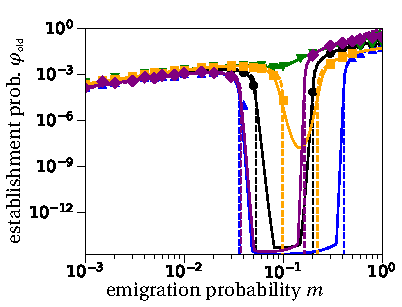
\includegraphics[width=\linewidth]{loglog_a.pdf}
  		\caption{$\varphi_{\text{old}}$ with $\omega_m = 1.35$ (large fecundity difference)}
	\end{subfigure}%
	\begin{subfigure}{.5\textwidth}
 		 \centering
 		 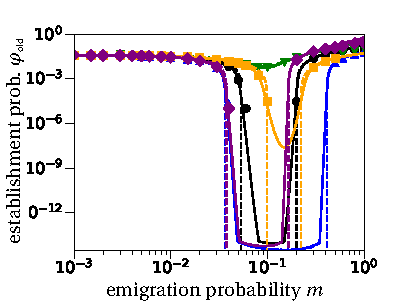
\includegraphics[width=\linewidth]{loglog_b.pdf}
  		\caption{$\varphi_{\text{new}}$ with $\omega_m = 1.35$}
	\end{subfigure}
    \caption{\textbf{Establishment probability on a log-log-scale.} This is Figure~\ref{fig:vary_m_est}(a,b) from the main text with the y-axis changed to a log-scale.}
    \label{fig:loglog}
\end{figure}

\begin{referee}
L330:\addnb{R1_30} Missing comma after $s_{\text{old}}$
\end{referee}
%
\st{When shortening the manuscript, this sentence was deleted.}\florence{We deleted the sentence as we shortened the manuscript. }

\begin{referee}
L372:\addnb{R1_31} Increases the population size relative to what? Pre-dispersal? Random migration? 
\end{referee}

In that paragraph we are discussing the differences between the New-New and New-Old dispersal schemes. Therefore, the increase in population size is relative to the New-New dispersal scheme. We clarified this (line~\ref{R1-31}).

\begin{referee}
L403:\addnb{R1_32} You can stay general and just give the $t_{\text{fin}}$ value used in the figure caption.
\end{referee}

We removed the corresponding sentence.

\begin{referee}
L421:\addnb{R1_33} You could mention this is because $P_{\text{adapt}}$ is essentially just $1-\exp(-C *\text{establishment})$, eq 8, with C a constant. 
\end{referee}

We followed the suggestion and added a sentence explaining this relationship (line~\ref{R1-33}).
\florence{(FD Not exactly true for Nnew)}
\begin{referee}
Fig3:\addnb{R1_34} Please give equation numbers for predictions (goes for all figures).
\end{referee}

We have \st{now }added references to the equations which we are plotting in the corresponding labels of the figures. \florence{[we have added / there are now]}

\begin{referee}
L441:\addnb{R1_35} Mention "soft sweeps". It might also be interesting to plot the probability of a soft sweep.
\end{referee}

We have added a brief reference to soft selective sweeps when discussing the origin of the rescue mutation, see lines~\ref{R1-35} and~\ref{R1-35-2}. The probability for a soft selective sweep in our context would be given by 
\begin{equation}
    1-\mathbf{P}(\text{no rescue}) - \mathbf{P}(\text{rescue from exactly one lineage}),
\end{equation}
which can be computed by the help of eq.~\eqref{eq:evol_rescue} and the Poisson distribution. The first two terms are simply the probability for evolutionary rescue and the last one is given by $\lambda \mathbf{P}(-\lambda)$, where $\lambda$ is the sum within the exponential in eq.~\eqref{eq:evol_rescue}. 

However, \florence{we do not provide this formula in the manuscript, because the manuscript is already long.}\st{ since we do not want to go into more details of soft selective sweeps (also due to the length of the manuscript), we do not provide this formula in the manuscript.} \florence{not soft sweep}

\begin{referee}
Eq9:\addnb{R1_36} You might want to note this is an approximation that assumes any mutation that has already established (or is on its way to establishing) does not interfere with the establishment of future mutations. Essentially it assumes all mutations establish at the same time (while they are all rare). Interesting to look at where the first establishing mutant is likely to arise (ratio of the rates)?
\end{referee}

The reviewer is correct in emphasizing that eq.~\eqref{eq:origin} is an approximation. The independence and non-interference of different mutant individuals and lineages is the basic assumption of \st{our whole methodology which relies on }branching process theory\florence{, the framework used in our study}. To emphasize this point yet again we have added a sentence around the description of eq.~\eqref{eq:origin} (line~\ref{R1-36}). 

Further, we agree that it is interesting to look at where the first establishing mutant is likely to arise which is given, as the reviewer points out, by the ratio of the dashed and the solid line in Figure~\ref{fig:origin}. However, since both values can take the value zero\florence{,} this ratio can not be computed over the entire x-axis\florence{,} which is why we did not plot the ratio. In fact, we had a similar discussion on this point \florence{among all authors} before our initial submission and \florence{had }decided to simply plot eq.~\eqref{eq:origin}. \florence{[not sure the In fact, ... sentence is necessary]}

\begin{referee}
L446:\addnb{R1_37} The surprise only arises when one tries to reason this out from the omega's rather than the s's, as it is relative fitness that matters most in the old environment and absolute fitness in the new environment. Framing this discussion around $s_{\text{old}}$ vs $s_{\text{new}}$ will be more intuitive (i.e. less surprising).
\end{referee}

\pete{hm... I am a bit confused. I could rephrase it in terms of $a_{\text{old}}$ but the surprise remains that even for large fecundity differences ($a_{\text{old}}\approx -0.1$ vs. $a_{\text{new}}=0.02$) a lot of successful mutant lineages emerge from the old habitat. Does anybody know what the referee means? I have deleted `surprisingly' (which also shortens the manuscript ;))} \florence{Then you can 1) remove "surprisingly", 2) explain here in the reply that things are still complicated/not straightforward when considering omega; 3) keep the text as it is (modulo "surprising")}

\begin{referee}
Fig4:\addnb{R1_38} I'd find it more interesting to sub out panel b for FigS3, which shows an example where the new patch contributes more.
\end{referee}
%
\st{Due to our change of fecundity values in the old habitat we do not observe the mentioned flip anymore.} \florence{The flip [or other word, I am not sure to understand what you mean by flip] does not happen anymore in FigXX with the updated fecundity values (changed following comment RefToCommentOnFecundities}. 
Therefore, we did not change the corresponding figure.

\begin{referee}
Eq10:\addnb{R1_39} I was confused for a while here because it is not made clear that $\varphi$ is now a function of $f_{\text{old}}$
\end{referee}

We have added a comment that we now consider the establishment probability to be a function of the frequency of old-habitat patches, see line~\ref{R1-39}. 

\begin{referee}
Eq10:\addnb{R1_40} I think the index inside $f_{\text{old}}$ should be $i+1$
\end{referee}

We adapted the definition of $f_{\text{old}}(i)$ such that now the correct old-habitat patch frequency is used (line~\ref{R1-40})\florence{[explain so that the AE does not need to check the text]}. The implementation of the formula in Figure~\ref{fig:rescue} was not affected by this mistake\florence{[typo or mistake?]}.

\begin{referee}
L470:\addnb{R1_41} Where is this deterministic population size calculated? Given this is an essential component of the probability of evolutionary rescue this should be given explicitly in the main text.
\end{referee}

\st{We are sorry that we did not provide the necessary equations in our initial submission. }We have now added a section in the SI, `Wild-type population sizes during the environmental change' (lines SXXff.) where we \st{state}\florence{provide} the equation for the deterministic population dynamics of the wild type in a changing environment\florence{ (sorry it was not included in the initial submission)}.

\begin{referee}
L473:\addnb{R1_42} What does "intersection" refer to? The y-axis, or each line with another?
\end{referee}

Intersection referred to the crossings of the different dispersal scheme lines. We now avoid using this term and rather speak of changes in the ranking of dispersal schemes, see also line~\ref{R1-42}.

\begin{referee}
L481:\addnb{R1_43} Can you state why you can't apply the Uecker result here? Can you apply the Uecker result to your RAND scheme? If so it might be nice to plot this in Fig5.
\end{referee}
%
Uecker et al. (2014) studied specific scenarios where a solution of the probability of evolutionary rescue was accessible, namely either $m=1$ or $\omega_m=0$. In these cases the branching process becomes one dimensional and the probability of establishment can be solved explicitly even in a time-varying environment. \florence{In our case, .... [explain why this is not the case for us]. }We now comment on this and give a bit more details, cf. line~\ref{R1-43}.

\begin{referee}
L497:\addnb{R1_44} Here viable is used in the more traditional sense, with non-viable meaning lethal (cf L80)
\end{referee}

We have changed the previous use of viable (see also our answer to comment~\comref{R1_9}) such that it \st{should be used coherently now} \florence{is now used consistently} throughout the manuscript.

\begin{referee}
L521:\addnb{R1_45} "were" ->  "where"
\end{referee}

We corrected the typo (line~\ref{R1-45}).

\begin{referee}
L525:\addnb{R1_46} Add a note about what changing tau does.
\end{referee}

We added a brief discussion about the effects of varying $\tau$, see lines~\ref{R1-46}ff.

\begin{referee}
Fig6a:\addnb{R1_47} As with Fig4, it would be more exciting to show a flip in the rank order of contributions (e.g. compare $\omega=9.9$ with $\omega=5$)
\end{referee}

Similar to Fig.~\ref{fig:origin}\florence{,} we do not longer observe a flip in the rank order of contributions \florence{because of}\st{due to }our new choice of fecundity values \florence{(a change suggested in comment REF [add ref to reviewer/AE comment])}.

\begin{referee}
Fig6b:\addnb{R1_48} If you plot this as a function of tau do you see a flip, i.e. at low tau SGV is more important than de novo while at high tau the opposite is true? 
\end{referee}

We have changed the time-intervals between consecutive deterioration events in Fig.~\ref{fig:sgv}(b). For $\tau=1$\florence{,} we see a flip of the contribution of de novo and standard genetic variation. Fort $\tau=5$ (results not shown)\florence{[show them here in the reply then - as a reviewer/AE I fight against "results not shown"...]} the effect of de novo mutants is again larger than that of standard genetic variation. 

\begin{referee}
L528:\addnb{R1_49} I think it's worth mentioning why: mutant spends most of the time in old patches.
\end{referee}

We restructured the sentence and now include the suggested wording (line~\ref{R1-49}). \florence{[are you sure about this? how is it compatible with high migration rates?]}

\begin{referee}
L529:\addnb{R1_50} It seems like the number before deterioration is a key aspect here, and this is not manipulated in Fig6b. Perhaps if theta is larger there will be enough mutants in the SGV that some establish, increasing the importance of SGV? This makes me wonder if you have tried to calculate the probability of rescue from SGV. For instance, you might just assume mutation-selection balance prior to the first deterioration event (giving N mutants across all M old patches) and then use $1 - \exp(-\varphi_{\text{old}}(f_{\text{old}}(1))*N)$ as the probability of rescue, where $\varphi_{\text{old}}(f_{\text{old}}(1))$ is the probability of establishment when there is just 1 new patch.
\end{referee}

\st{We had the same idea as the referee. However, }\florence{Unfortunately, }this formula does not capture the probability for rescue due to standing genetic variation since the probability of adaptation for a mutant individual initially in an old-habitat patch is equal to zero (or at least very close to it) over the whole parameter range of the emigration probability $m$ (see the new Fig.~SXX in the SI). Additionally, in the scenario where standing genetic variation is most likely to affect the probability of evolutionary rescue, i.e. for a fast environmental change (small $\tau$), the suggested approximation does not take into account the environmental change which is crucial for an evolutionary rescue event to happen from standing genetic variation. \florence{[that's additional work but maybe you could plot the suggested formula, and put the figure here to illustrate that it does not work?]}

\begin{referee}
L540-547:\addnb{R1_51} I'm a bit confused here. You state that population size in each patch is constant regardless of dispersal (L541) but then say that more dispersal leads to more non-adapted individuals in the new environment (L546). 
\end{referee}

The population sizes after the whole life cycle remain constant at the respective carrying capacity.\florence{[specify when/under which conditions, otherwise they may this is all the time]} After dispersal the number of individuals may be above the carrying capacity but after reproduction and density regulation the population is again at the initial value. In our scenario the population sizes may be below the carrying capacity even after reproduction and density regulation\florence{[hmm need to reformulate the reply because this seems to contradict the first sentence]}. We added a brief comment in line~\ref{R1-51}.

\begin{referee}
L563:\addnb{R1_52} Replace "Dispersal" with "Standing genetic variance"
\end{referee}

We changed the title of that section following the suggestion (line~\ref{R1-52}).

\begin{referee}
L589-591:\addnb{R1_53} Needs elaboration or drop.
\end{referee}

\pete{I am happy to drop these three lines. The part in the SI (Section S6) can stay without further explanation I think. }\florence{[no strong opinion on this - maybe drop to shorten?]}

\begin{referee}
L596:\addnb{R1_54} This also seems important once more loci are considered, both for the case of neutral and deleterious hitchhikers (i.e. does the rescue mutation arise on an "old" or "new" haplotype) as well as in sexual populations where mutations at multiple loci are required for rescue (in which case depending on the "old" and "new" haplotypes recombination could help or hinder rescue). Is it worth adding a paragraph about sex/recombination/polygenic rescue here? Also makes sense after L640.
\end{referee}

We have added a brief reference to this area of research but do not want to go into the details of the rescue process in these situations (line~\ref{R1-54}). We think that more explanations would be needed and decided to not extend the manuscript length any further (see also the general comments of the two editors).
\pete{I think if we make more than a reference we need to go deeper into explanations of how rescue works in these situations which I would like to avoid. How do you feel about that? Maybe add another reference -- Hildegard, do you know something off the top of your head?}

\hildegard{Have a look at the abstracts. Not sure they are suitable to cite in the context.}
\begin{itemize}
    \item Schiffers, K., E. C. Bourne, S. Lavergne, W. Thuiller, and J. M. J. Travis, 2013 Limited evolutionary rescue of locally adapted
populations facing climate change. Philos. Trans. R. Soc. Lond.
B Biol. Sci. 368(1610): 20120083.
    \item Bourne, E. C., G. Bocedi, J. M. J. Travis, R. J. Pakeman, R. W.
Brooker et al., 2014 Between migration load and evolutionary
rescue: dispersal, adaptation and the response of spatially structured populations to environmental change. Proc. Biol. Sci. 281
(1778): 20132795.
    \item Pease, C. M., R. Lande, and J. J. Bull.1989. A model of populationgrowth, dispersal, and evolution in a changing environment. Ecology 70:1657--1664.
    \item Polechov{\'a}, J., N.H. Barton, and G. Marion. 2009. Species'
    range: adaptation in space and time. American Naturalist 174:E186--E204.
    \item Duputi{\'e}, A., F. Massol, I. Chuine, M. Kirkpatrick, and O.  Ronce.2012. How do genetic correlations affect species range shifts in achanging environment. Ecology Letters 15:251--259.
\end{itemize}

\begin{referee}
L600-604:\addnb{R1_55} As stated in my comment about L164, the assumptions of ABS should be laid out very clearly: the mutant migrates to habitat patches where it has lower fitness (except if m is really large). This is lost here, where the authors state "habitat choice protects a population against locally deleterious mutations" -- which is only true when the mutations migrate to patches where they have lower fitness. This clear explanation should be stated. \\

L611:\addnb{R1_56} If the trait is not which type of patch to enter (here acting like ABS) but to enter the patch one is best at (here REL) this trait does not have to evolve, but perhaps this "all-seeing" trait is unlikely to exist...\\

L613:\addnb{R1_57} Can you say a few more words about the ciliates? e.g., what were the habitats, how fast did preference evolve?
\end{referee}

In our attempt to shorten the manuscript we deleted the section ``Evolutionary consequences of habitat choice'', which the\florence{se} \st{previous }comments refer to.

\begin{referee}
L622 and L632:\addnb{R1_58} I'm a bit confused here as $s_{\text{old}}$ is not constant in time. Perhaps you mean constant between deterioration events? But even then you say population dynamics are changing (L470). 
\end{referee}

Indeed, as the referee mentions, the population size changes\florence{[need to discuss this as I am not sure to understand: doesn't it change all the time anyway?]} when we consider the evolutionary rescue scenario which in turn alters the parameter $a_{\text{old}}$\florence{(previously written  $s_{\text{old}}$)}. However, \florence{we approximate xxx as constant between two deterioration events. }in the analysis we assume $a_{\text{old}}$ to be constant between two deterioration events (which is the major reason for the \st{disagreement}\florence{difference/discrepancy/other term?} of our approximation and the simulation results, see line~\ref{R1-58-2}). We now specify what we mean by constant parameters by highlighting that this does not necessarily hold in our rescue situation (line~\ref{R1-58-1}).

\begin{referee}
L646:\addnb{R1_59} Is this a general framework or an application of multi-type branching processes?
\end{referee}

\pete{I would argue that our framework is very general when it comes to modeling populations in discrete time since we can vary basically all parameters and add/remove steps in the life-cycle arbitrarily. I agree that the analysis is an application of multi-type branching processes but the model itself is very general.}\florence{[fine with me]}

\begin{referee}
L656:\addnb{R1_60} Better to give example of dispersal scheme that hinders rescue first (to follow up on your previous sentence). I think it is also important, throughout the Discussion, to spell out what the schemes are, i.e. to say that "negative density-dependent" dispersal means the mutants migrate to patches where they have higher fitness and the wildtypes do the opposite.
\end{referee}

We deleted the sentence since we believe that throughout the manuscript we have made our point clear that non-uniform dispersal can alter the evolutionary outcome.

\begin{referee}
EqS7\addnb{R1_61} (and many equations that follow): $f$ should be $f_{\text{old}}$\\

LS35:\addnb{R1_62} $\pi$ should be $\pi_w$
\end{referee}

\st{We are very sorry for this shortcoming.}\florence{Thanks for noticing.} We corrected both typos in all the formulas (and also changed $\pi_w$ to the newly defined $\widehat{\pi}_w$).

\begin{referee}
LS38:\addnb{R1_63} should be equation 2, not 3 (all equation references to the main text are wrong in the SI too)
\end{referee}

Unfortunately, this was due to the same mistake\florence{[compilation error on the website?]} that led to the wrong numbering in the main text, see also comment~\comref{R1_12}. This problem is resolved now. 

\begin{referee}
LS44:\addnb{R1_64} It is not that you "do not assume density regulation" but that you assume no density-dependence
\end{referee}

We rephrased the sentence (line~SXX).

\begin{referee}
LS53:\addnb{R1_65} Add comma after $s_{\text{old}}$
\end{referee}

Corrected.\florence{[this review would be so much more pleasant to read if they had written some "please" instead of given orders like this!]}

\begin{referee}
eqS17:\addnb{R1_66} Where do you prove that the branching process is only "slightly" supercritical? Is this implied by zeta and mu being small in this equation?
\end{referee}

The process is slightly super-critical because for $\varepsilon\to 0$ the eigenvalue converges to $1$ (cf. eq.~(SXX)). This translates to the rates $a_{\text{old}},a_{\text{new}}$ and $m$ being very small which is modeled by their scaling with $\varepsilon$. We added a bit more details in the corresponding section to highlight this (lines~SXXff.).

\begin{referee}
LS91:\addnb{R1_67} "We now proceed to explain"
\end{referee}

We rephrased the sentence following the suggestion (line~SXX).

\begin{referee}
LS103:\addnb{R1_68} Again, relative fitness in the new patch is irrelevant, it is absolute fitness that matters
\end{referee}

\st{This is entirely right. W}\florence{We agree and w}e adjusted the phrasing accordingly, see line~SXX.\florence{[do we? I cannot check because I do not have the SI with line numbers...]}

\begin{referee}
FigS1 and EqS20 and L301: \addnb{R1_69} Worth mentioning that $\varphi_{\text{old}}$ is zero when $m=0$ (in contrast to $\varphi_{\text{new}}=2s)$? When I first saw FigS1c I thought term 1 and 2 must be driving the patterns because they are so much larger in absolute value than term 3, but then I saw from EqS20 that they must exactly cancel at small enough m.    
\end{referee}

We have added a brief sentence in the main text (line~\ref{R1-69}) and also in the SI (lines~SXX) to highlight that terms (1) and (2) cancel for $m=0$.

\begin{referee}
FigS1cd:\addnb{R1_70} Would it be clearer to plot REL rather than RAND if you are interested in regime ii?
\end{referee}

We have followed the suggestion. Unfortunately, still the local maximum is not well visible in these figures due to the scaling of the y-axis which is necessary to capture terms (1) and (2).\florence{[so does it make sense to follow the suggestion?]}

\begin{referee}
LS153:\addnb{R1_71} So you are now assuming hypergeometric sampling rather than independent Poisson processes, right?
\end{referee}

Since we have changed the dynamics in the old habitat to follow the same rules as in the new habitat (fecundity modeled by a Poisson distribution and then down-regulation by hypergeometric sampling) this also applies to the scenario without demography.\florence{[I do not understand the sentence - think about the AE, put the reply back into context so that the AE does not have to check the paper to understand what this is about. It is longer to write but pays off because a happy AE is more likely to accept your paper!]} (For our chosen population sizes $K_{\text{old}}=K_{\text{new}}=500$ and fecundities $\omega_k^i\approx 1.5$ the carrying capacity is always reached with high probability.)

\begin{referee}
EqS21:\addnb{R1_72} These could just be given in the figure caption, no? Or does this impact eq S22 and S23?
\end{referee}

As suggested, we have moved the fecundity values to the caption of Figure~SXX. 

\begin{referee}
L163:\addnb{R1_73} This isn't really highlighted in the main text, instead L561 just refers readers back to this SI. Perhaps more detail should be moved to the Discussion?
\end{referee}

We changed the word ``highlighted'' in the SI (line~SXX). We refrained from adding more details about the reason for the different outcomes in region (iii) between models with and without demography in the main text because \st{we do not visualize them there} \florence{this is not where they are seen (they are in figXXX)}. Instead we leave the detailed discussion, as it was before, in the SI. 

\newpage
\refsec{Reviewer \#2:}

\begin{referee}
This\addnb{Ref2Intro} is an interesting paper on effects of different kinds of dispersal on evolutionary rescue. The habitat consists of a number of patches which start out with a favorable environment but each in turn deteriorates. The organism has two types (wild type favored in the original environment, mutant type favored in the degraded environment) that reproduce clonally. Each type can have unbiased dispersal or dispersal biased toward one habitat type (the one they have greater absolute or greater relative fitness). Branching processes are used for approximate analytical results and complemented by simulations. Dispersal magnitude and type affects the probability that a mutant arrives in the degraded habitat (where a lineage must persist for rescue) and the distribution of the wild type, which affects the fitness of the mutant in patches that have not yet degraded. These both contribute to rescue, of course. 

Previous evolutionary rescue papers often assume either a single abrupt change in the environment or a continual linear change (sometime with random variation around one of these). This paper uses a step-wise change that has features of each (spread out over time like the continual change, but limited in total magnitude of change like the abrupt change). In deriving the evolutionary rescue results, the paper also uses analyses of source-sink systems, since between the starting and ending states there are both good patches (sources for the wild type) and bad patches (sinks). The authors reference species in natural systems that match many of their assumptions.\\

\vspace{-10pt} Specific comments (\_ indicates that what follows is a subscript, and \^{} a superscript). \\

line 4.\addnb{R2_1} Change 'wild-type population' to 'population whose wild type is'.
\end{referee}

We changed the wording as suggested (line~\ref{R2-1}).

\begin{referee}
line 45\addnb{R2_2} (and other places). Change 'the other' to 'another' ('the other' suggests that there are only 2).
\end{referee}

We followed the suggestion and changed all these occurrences of `the other'.

\begin{referee}
line 49.\addnb{R2_3} Add 'increasing' before 'dispersal' if this is what you mean, since the current wording suggests that the comparison is between systems with and without dispersal.
\end{referee}

We clarified the sentence by adding `increasing' (line~\ref{R2-3}).

\begin{referee}
line 54.\addnb{R2_4} Using 'random' to mean 'with a uniform distribution' is common but I would use random to mean the opposite of deterministic, for example constant, dispersal. Later, the paper mentions biased dispersal, so I think it would be better to use 'unbiased' instead of 'random'.
\end{referee}

When changing the range of the dispersal bias parameters $\pi_w$ and $\pi_m$, we also changed the names of the dispersal schemes (compare also our response to \comref{AE2}). In \st{alignment}\florence{line} with this, we also replaced all the occurrences of `random' by either `uniform' or `unbiased'. \florence{Thanks for the suggestion.}

\begin{referee}
line 74.\addnb{R2_5} I would change 'for an individual to leave' to 'that an individual leaves'. I think this same construction occurs elsewhere (sometimes with probability instead of likelihood), and I would change those also.
\end{referee}

\st{We are very grateful for the plenty stylistic comments made by the reviewer. If not mentioned differently, w}\florence{W}e followed the \florence{reviewer's}suggestions \st{of the him/her in all cases}\florence{and thank her/him for them. [NB: `the rule, at least in French, is to list options alphabetically, so her/him]} (comments \comref{R2_17}, \comref{R2_23}, \comref{R2_24}, \comref{R2_36}, \comref{R2_38} and \comref{R2_41}).

\begin{referee}
lines 95-96.\addnb{R2_6} I would write that in old-habitat patches both types have a mean reproduction >  1 with the wild type being higher, and there is ceiling density regulation (only K individuals reproduce in each patch each generation). 
\end{referee}

We have changed the initial description of the model in the spirit of the suggestion, lines~\ref{R2-6}ff.

\begin{referee}
lines 108-109.\addnb{R2_7} Change 'amount of offspring that is' to 'number of offspring that are'.\\

line 121.\addnb{R2_8} 
Add 'so the number of mutants is determined using' before 'a binomial'.\\

lines 123-124.\addnb{R2_9} Change '(wild-type individuals turning into mutants)' to '(probability that an offspring of a wild-type individual is a mutant)'.
\end{referee}

\florence{[maybe use one number for the three lines then (i.e. just R2-7, and jump to R2-10 later), otherwise it first looks like you have ignored the comments]}
Since we have changed the fecundity values in old-habitat patches to be a lot smaller than before (compare \comref{AE4} and \comref{R2_22}) we now model the dynamics in these patches differently so that the phrasing has changed and these comments do not apply anymore, see lines~\ref{R2-7}, \ref{R2-8} and \ref{R2-9}. Briefly, we now model the population in old habitats in the same way as in new habitats, i.e. we first assume reproduction by drawing a Poisson number of offspring for each individual and then we regulate the population size (if necessary) by sampling hypergeometrically, that is, without replacement.\florence{[Maybe make this really clear above as well!]}

\begin{referee}
equation (2).\addnb{R2_10} Using equation (1), the denominator would have '$+ \omega_m$' at the end. If this is assumed to be negligible, that should be stated. This also applies to equation (S22).
\end{referee}

We have added an explanatory sentence at both approximations (lines~\ref{R1-11} and SXX\florence{; yes it is assumed to be negligible [if true]}).

\begin{referee}
line 131.\addnb{R2_11} 'eq. (3)' here should be 'equation (2)'. From this point on, very many (perhaps all) of the equation numbers are 1 too high. So these all need to be corrected.
\end{referee}

We are very sorry for this \st{blunder}\florence{compilation issue} and resolved it.

\begin{referee}
line 134.\addnb{R2_12} It is not clear what $N_w^{\text{old}}$ refers to here. Is it the total over all old habitats, and at what point in the life cycle?
\end{referee}

There was a tilde missing above the variable (see also \comref{R1_13}). We now specified the point in the life cycle and that it is the average wild-type population size in one single patch (line~\ref{R2-12}).

\begin{referee}
lines 145-146.\addnb{R2_13} Some of the equations (such as [S5]) can have new patches at K.
\end{referee}

This is true. However, to simplify the analysis we assume density-independent reproduction in new-habitat patches\florence{,} which is reasonable as long as the carrying capacity is not reached. In the simulations\florence{,} the carrying capacity might be reached\florence{,} in which case our approximation fails (this partly explains the worse fit for large frequencies of old-habitat patches, $f_{\text{old}}$). We now provide more details explaining this point, cf. lines~\ref{R2-13}ff.

\begin{referee}
lines 151ff.\addnb{R2_14} Delete 'The bias of immigration into new-habitat patches is set equal to one, without loss of generality.' I think $\pi_i$ is the ratio of the probability of entering a specific old patch to that of entering a specific new patch for type i. If so, it should be defined in that way, since 'bias in immigration' is less clear.
\end{referee}

We have changed the meaning of the parameter $\pi_i$ (see also comments \comref{AE2} and \comref{R1_19}). Now, $\pi_i$ is indeed a bias, and the value in the formulas is given by $\widehat{\pi}_i=e^{\pi_i}$. As such, we continue describing $\pi_i$ as a bias. Still, we rephrased parts of the corresponding paragraph to be more clear about the meaning of $\pi_i$ and $\widehat{\pi}_i$ (lines~\ref{R2-14}ff.). 

\begin{referee}
line 161.\addnb{R2_15} The equation for this is (S2), and it is not that clear how this is analogous to (3), so I think the equation should be given (or refer to the supplement if it is not important for the main text).
\end{referee}

We have simplified the dispersal notation since emigration is independent of the type of the individual and also the habitat-type (cf. comment~\comref{R1_21}). Now both dispersal rates, into new and into old habitats are given in the main text, see eq.~\eqref{eq:dispersal}.

\begin{referee}
lines 164-166.\addnb{R2_16} Obviously, it is being assumed that $\omega_m >  1 + s_{\text{new}}$, but that should be stated explicitly. 
\end{referee}

We followed the suggestion and now explicitly state the assumption underlying this dispersal scheme (line~\ref{R2-16}).

\begin{referee}
line 211.\addnb{R2_17} Change 'been using' to 'used'.\\
\end{referee}
\florence{done [otherwise it looks like you have omitted the comments; they won't remember that you listed the number above]}

\begin{referee}
lines 216-219. \addnb{R2_18} This needs to be explained in more detail. There are 10 patches and 2 types, so I presume 20 random numbers of dispersers were picked, one for each type in each patch, and the population size of each type in each patch decremented by that number. For each type, the dispersers from all patches can be summed, and then the number that go to each patch type can be determined using a binomial with p value determined by the $\pi_i$ value for that type and $f_{\text{old}}$ (the fractions in eqq. [S1] and [S2]). Then, these dispersers can each be added to a patch of the appropriate type (I assume randomly with equal probabilities). I would also cut 'Then reproduction happens locally.', because in old-habitat patches, reproduction, mutation and density regulation are done together. 
\end{referee}

We have added more details when describing the dispersal step in the simulations, see lines~\ref{R2-18}ff. We also followed the suggestion of cutting `Then reproduction happens locally' since the next sentence now begins with `In each patch...'.

\begin{referee}
lines 221-224.\addnb{R2_19} The Poisson distributed number for each type is the product of its mean offspring number and the number of adults of that type. I would also start with 'In each new-habitat patch' and change 'both types' to 'each type' [so there are $2(1-f_{\text{old}})$ Poissons if each new-habitat patch has both types]. 
\end{referee}

We have rephrased the corresponding sentence to clarify the mean of the Poisson numbers that we draw randomly (lines~\ref{R2-19}ff.). It depends on the type of the individual giving birth, the number of those individuals in the focal patch and the patch type.

\begin{referee}
line 224.\addnb{R2_20} Change 'individuals' to 'offspring' and 'rate' to 'probability'.
\end{referee}

We followed the suggestion (line~\ref{R2-20}).

\begin{referee}
lines 232.\addnb{R2_21} Add 'over a finite time period' after 'mutations'. Also, since this paragraph is stated to be about figures 2-4, it would be better to write 'figures 3-4' instead of 'all the other figures'.
\end{referee}

We followed both suggestions and rephrased the sentence accordingly, see line~\ref{R2-21}.

\begin{referee}
Table 1.\addnb{R2_22} It appears that $s_{\text{new}}$ was chosen so that the approximation in (6) is valid, and the values of $\omega_m$ so the mutants in the source to be determined by a binomial using (1). It is a little odd that the mutant goes from a birth rate of at least 9 in the old habitat to 1.02 in the new habitat. The results obviously would be vastly different if the latter were a little lower. With a birth rate of 1.02, each mutant lineage in the new habitat has a high probability of going extinct, and the result could be significantly different if the new habitat birth rate were not so close to 1.
\end{referee}

We now reduced the average number of offspring in old-habitat patches to $\omega_w=1.5$ and $\omega_m=1.35$ or $\omega_m=1.45$ dependent on the studied fecundity difference to the wild type (see also comment~\comref{AE4}). For these values our approximation is still applicable (preliminary simulations suggest that $\omega_m=1.1$ still gives reasonable results). \st{Concerning the choice of the local growth rate of the mutant in new-habitat patches w}\florence{W}e followed the previous choices made in Uecker et al. (2014) and more recently in Tomasini \& Peischl (2019+)\florence{ for the [value of the?] local growth rate of the mutant in new-habitat patches [try to avoid ``Concerning..., ...'']}. The particular choice of $1.02$ is interesting since for this choice of parameters we observe a local maximum in the establishment probability when varying the emigration probability and the mutant fecundity in the old habitat (Figure~2). \hildegard{The last sentence sounds as if we tuned the parameters and it is really important to have 1.02 to obtain the results. I think it is mainly important that it is small enough such that rescue is not guaranteed. Which pattern we observe also depends on the mutant fitness in the old habitat. If this is low, the fitness in the new patches can be larger, and we still see a maximum.}\florence{+1, the phrasing makes it sound like this is an exceptional event, only happening at this value} If we increase the local growth rate in the new habitat\florence{,} the local maximum disappears since we increase the positive effect due to dispersal (term (3)) and the local growth rate in new habitats (term (1) in $\varphi_{\text{new}}$) (see also our response to comment~\comref{AE5}  from the associate editor).

\begin{referee}
line 253.\addnb{R2_23} I would change 'where' to 'after'.%\\
\end{referee}
done
\begin{referee}
line 261.\addnb{R2_24} Change 'evolve' to 'reproduce, disperse and die' or something like that - individuals do not evolve.%\\
\end{referee}
done
\begin{referee}
line 264.\addnb{R2_25} Add 'total' before 'numbers' if that is the meaning. Also, specify the point in the life cycle at which $N_m^k$ is defined.
\end{referee}

We have rephrased that sentence in order to clarify the two-type branching process, see line~\ref{R2-25}.

\begin{referee}
line 271.\addnb{R2_26} I would add '(see SM1 for the derivation of $s_{\text{old}}$ at the wild-type equilibrium)' after the equation number (which should be 2).
\end{referee}

We followed the suggestion and added the reference to the SI (line~\ref{R2-26}).

\begin{referee}
top of page 15.\addnb{R2_27} See comments on lines 102ff in the supplement on the interpretation of the terms in these equations.
\end{referee}

Our explanation in the main text is intentionally very heuristic and not focused too strongly on the formula. In the SI, we \st{now }added \florence{/now provide} more details on the effects of the dispersal rate on the single terms of the establishment probability, see also our response to comment~\comref{R2_50}.

\begin{referee}
line 298.\addnb{R2_28} Add '(see SM1)' at the end.
\end{referee}

We added the reference as suggested (line~\ref{R2-28}).

\begin{referee}
line 309.\addnb{R2_29} Add 'in the old habitat' after 'reproduction'.
\end{referee}

The approximation of the establishment probability deviates for both estimates, $\varphi_{\text{old}}$ and $\varphi_{\text{new}}$, for large values of the emigration probability $m$. Therefore, we did not change the sentence.

\begin{referee}
lines 327-328.\addnb{R2_30} I would change 'larger amounts of mutant individuals that, once emigrated to a new habitat, reimmigrate into an' to 'a larger probability that an individual born in a new habitat migrates to an'. As I understand the model, individuals can only migrate once, so individuals don't migrate and then re-immigrate. Also, extinction is most likely when there is only one mutant, so I think it is better to frame this statement in terms of probability rather than numbers. ('Re-immigrate' is used elsewhere also, and it would be better to re-word these passages to avoid this term, or make explicit that it is a lineage, or descendant, that re-immigrates.)
\end{referee}

We agree with the reviewer in all points and have changed the wording accordingly.\florence{[re-immigration makes sense where talking about a lineage, doesn't it? I think it is still an interesting perspective to have and suggest talking about lineages - i.e. differentiate between what happens to individuals (cannot reimmigrate) and lineages, and mention both. What do you think?]} We now avoid speaking of re-immigration since indeed an individual only migrates at most once before its death (lines \ref{R2-30-3} and \ref{R2-30-4}). We also followed the suggestion to speak of migration probabilities rather than proportions of individuals (line~\ref{R2-30-1}) since this is indeed, as the reviewer points out, the crucial point.  

\begin{referee}
Figure 2\addnb{R2_31} legend, third line. Add 'symbols' after 'simulations' (assuming that is correct). 
\end{referee}

As suggested, we added `(symbols)' to clarify that simulation results are depicted as the different symbols.

\begin{referee}
lines 332-333.\addnb{R2_32} I would change 'number of mutants in the new-habitat patches through back-migration' to 'probability that a mutant migrates from new to old habitat'. It would be good to point out that the expected number of offspring of a mutant in new habitat that remain in new habitat is the product of $1 + s_{\text{new}}$ and $1 - m^{(\text{new}\to\text{old})}$, the latter of which increases with m. For high enough m, this can be less than 1, in which case persistence requires descendants of mutants that leave migrate back into new habitat at a rate sufficient to make up for the deficit, which is unlikely (assuming that the reproduction number is less than 1 in old habitat also). This probably explains the 0 values for establishment rate in some of the figures, even when the mutant starts in new habitat. 
\end{referee}

We agree with the reviewer and therefore changed the phrasing to the suggested form. We also added a more details on the mechanism as described by the reviewer, see lines~\ref{R2-32}ff.\florence{[please see comment above \comref{R2_30}]}

\begin{referee}
lines 378-379.\addnb{R2_33} Remind the reader that with absolute habitat choice, both types prefer the old habitat, so the behavior of the wild type is the same and the mutant type the opposite than with relative habitat choice. This generally leads to lower establishment than the other so far discussed, because the mutant behavior is maladaptive (which also explains the similarity to the maladaptive curves noted in the next paragraph). The exception is the case you note, in which the mutant does better in old habitat at high m, in which absolute habitat choice can lead to higher establishment than relative habitat choice.   
\end{referee}

Since we have changed the names of the dispersal schemes to the corresponding preference, i.e. `Old-Old' for both types having a bias towards the old habitat, we think that we do not need any further reminder concerning the dispersal preferences.

\begin{referee}
lines 407-408.\addnb{R2_34} If only mutants arising in old habitat are considered, I think the probability of adaptation should be the probability that a binomial with parameters $M*f_{\text{old}}*K*t_{\text{fin}}$ (number of offspring that survive density regulation) and $\theta*\varphi_{\text{old}}$ (probability that a birth produces a mutant whose lineage survives) is 0. A Poisson should give a very good approximation, but assuming it is an approximation, that should be stated. (The situation is more complicated for mutants arising in new habitats, because the number of wild-type individuals is a random variable with I think a complicated distribution.)
\end{referee}

We added a \st{very brief }comment\st{, not going into too many details,}\florence{} that using the Poisson distribution is indeed, as the reviewer correctly pointed out, an approximation (line~\ref{R2-34}). 

\begin{referee}
lines 421-422.\addnb{R2_35} It could be pointed out that there are some differences in the order in panel (c) that likely results from effects of dispersal type on the equilibrium $N_w^{\text{new}}$. 
\end{referee}

We have added a \st{brief }\florence{}comment where we point out that the small differences between Fig.~\ref{fig:vary_m_est}(c) and Fig.~\ref{fig:source_sink}(c) in terms of the ranking of dispersal schemes goes back to the equilibrium sizes of the wild type in new-habitat patches, as pointed out by the reviewer (cf. lines~\ref{R2-35}ff.).

\begin{referee}
lines 441-3.\addnb{R2_36} Add 'at least' before 'one' and change 'a mutant from an old-habitat patches' to 'mutants from old-habitat patches only'.\\

lines 446-448.\addnb{R2_37} It is helpful in explaining this to note that the rate at which successful lineages are generated in each habitat type is proportional to $\varphi_i*f_i*N(hat)_w^i$. If figure 4(a), adaptation requires $f_{\text{old}} < 0.5$, and is higher for old habitat even for $f_{\text{old}} = 0.1$. The reason must be much higher values in old habitat of either or both of the equilibrium wild-type population (larger in old habitat) and the probability of establishment of a mutant in each habitat. Plots of those as a function of $f_{\text{old}}$ would be helpful here. Unfortunately, although $\varphi_i$ is plotted as a function of $f_{\text{old}}$ in figure S4, that figure uses a much higher m. $N(hat)_w^{\text{new}}$, however, seems to be about 2-7\% of K for the points in (a), if my calculations are correct.
\end{referee}

In order to disentangle the effects of population size and establishment probability on the origin of the successful mutant we now plot both values when varying the frequency of old habitats, $f_{\text{old}}$ (see Fig.~SXX in the SI). Indeed, the mutational input which is scaled by the population sizes in the corresponding patches seems to be responsible for the dominance of the old habitats concerning the origin of the rescue mutant. 

We also added a brief explanation in the main text (lines~\ref{R2-36}ff.) and refer to the figure in the~SI.

\begin{referee}
line 456.\addnb{R2_38} Change 'unevitably' to 'inevitably'.%\\
\end{referee}
\florence{done}
\begin{referee}
equation (10).\addnb{R2_39} I think i should go from 0 to M - 1 and the last summation should start at M*tau. For M - 2, the limit of i in the equation, $f_{\text{old}} = 2/M$, but the last term has $f_{\text{old}}$ (the argument of $\varphi_{\text{new}}) = 0.$ So $f_{\text{old}} = 1/M$ is missing. The various terms in the exponential give the expected number of mutants arising at each time whose lineage survives. This should peak at intermediate values, because for high $f_{\text{old}}$ the rate of mutant generation is high but the lineage persistence is low, and the opposite is true for low $f_{\text{old}}$. In the middle, both are intermediate and so that product likely reaches a maximum for intermediate $f_{\text{old}}$, such as seen in figure 3b,d. This is relevant to the results for standing variation, because the lineages of initially present mutants must survive hostile conditions until $f_{\text{old}}$ drops at least to 0.8 (as implied by fig. 3d for conditions in fig. 6b).
\end{referee}

The frequency of old habitats, $f_{\text{old}}(i)$, was \st{wrongly}\florence{inaccurately} defined (see also \comref{R1_40}). We corrected \st{that mistake}\florence{it}\st{ so that the formula should be correct now} (eq.~\ref{eq:evol_rescue}). We also added the explanation that the reviewer is giving for the low impact of standing genetic variation around Figure~\ref{fig:sgv} (line~\ref{R2-39}).

\begin{referee}
Figure 5\addnb{R2_40} is based on equation (10), which is approximate. However, as in most other figures, there is a curve labeled 'exact'. I think the meaning is a numerical solution of equation (5) is used for $\varphi_i$ rather than the approximate values in equation (6). It should be made clear that exact refers only to $\varphi_i$, not the whole curve.
\end{referee}

We now clarify in the caption of Figure~\ref{fig:rescue} that the label `exact' refers to the exact solution of eq.~\eqref{eq:ext_prob}. 

\begin{referee}
line 470.\addnb{R2_41} Add 'expected value of' after 'follow'.%\\
\end{referee}
\florence{done}
\begin{referee}
lines 474-479.\addnb{R2_42} I think it would be better to write that the approximation assumes that a mutant has the establishment probability assuming the environment is fixed for the environment ($f_{\text{old}}$) in which it is born (and I think also at the equilibrium population sizes for that environment). In the initial environment, the rate of creation of mutants is high but the establishment rate is low (0), and as deterioration progresses, the former decreases and the latter increases. The approximation captures the decrease in mutant creation but not the increase in establishment probability of a mutant whose lineage experiences a change in the environment (which as the paper states is likely for a mutant arising just before a change). 
\end{referee}

In line with the reviewers comment we now explain more explicitly which assumptions of the establishment probability $\varphi_k$ are violated in the evolutionary rescue situation, cf. lines~\ref{R2-42}ff.

\begin{referee}
lines 486-489.\addnb{R2_43} The wording here is not clear. It might be better to state something like negative density-dependent is higher than random which is higher than absolute habitat choice, with relative habitat choice decreasing and maladaptive dispersal increasing their positions with increasing m. 
\end{referee}

We followed the suggestion of the reviewer and rephrased the sentence accordingly (lines~\ref{R2-43}ff.).

\begin{referee}
lines 489-491.\addnb{R2_44} I assume this means that $s_{\text{old}}$ is the most influential factor in the change in position of relative and maladaptive dispersal, but if so this should be made clear. The relative position of the other three strategies I think depends on mutant dispersal probability into new habitat. 
\end{referee}

The reviewer is correct in \st{his/her}\florence{[alphabetical] her/his} assessment. We changed the wording, now differentiating between the ranking of the symmetric dispersal schemes and the change of the order for the asymmetric schemes, lines~\ref{R2-44}ff.

\begin{referee}
lines 527-529.\addnb{R2_45} Before the first degradation event, all patches are old, and I think dispersal is irrelevant. There should be an expected equilibrium number of mutants in each patch given by the solution of $X_{\text{mut}} = K p_m$, where $p_m$ as given in equation (1) with the number of mutants equal to $X_{\text{mut}}$ and the number of the wild type $= K - X_{\text{mut}}$. So the standing genetic variance should not depend on m. One reason (perhaps the major one) for the drop in the relative contribution on standing variation with increasing m is the fact that the rescue probability increases with increasing m, by a factor of about 10. If the number of populations rescued by mutants from the standing variation didn't change with m, this would cause the relative contribution to decrease by a factor of 10. Of course, once the first patch deteriorates, the loss of lineages from standing variation mutants does depend on m, but I would guess higher m is better, since it gets more mutants into the new patch and might relax competition in the old patches a little.
\end{referee}

\florence{[maybe you can subdivide the point? what about the first sentence btw?]}
The referee correctly points out that the probability of establishment after the first degradation changes with $m$. We have added a Figure in the SI to highlight this, see Fig.~SXX. There we plot the establishment probabilities $\varphi_{k}$ for varying emigration rates $m$ in the setting where one patch has deteriorated ($f_{\text{old}}=0.9$ in our standard parameter set). This is the environment which the mutants experience at time $t=0$. It can be seen that increasing $m$ indeed does not change the probability of establishment for mutants in old-habitat patches. It is in fact very close to $0$. Yet, for the mutants in the patch that deteriorates first, the establishment probability decreases with increasing $m$ for most dispersal schemes. Furthermore, for very large values of $m$ we enter the gene swamping scenario which also inhibits the establishment of mutant lineages in the new habitat. 

Therefore, we are still convinced that our argument, for increasing dispersal rates the effect of standing genetic variation becomes less important for the overall rescue probability, remains valid. %To further validate this, we now also plot the effect of standing genetic variance for smaller values of $\tau$, the time between two consecutive deterioration events (see Fig.~\ref{fig:sgv}(b)). Here, the probability of evolutionary rescue (from de-novo mutants) changes less than the impact of standing genetic variation does \todo{figure!}. 

\begin{referee}
line 545.\addnb{R2_46} 'Gene swamping' is often used for populations with sexual reproduction. In this case, dispersal can inhibit adaptation in a source-sink system because source individuals dispersing to the sink mate with each other but also with individuals in the sink. Therefore, if an adapted type arises in the sink but is still rare, it is likely to mate with an immigrant, which is maladapted in the sink. Their offspring will often be much less fit in the sink than the adapted parent, inhibiting adaptation. This factor is not present with clonal reproduction.   
\end{referee}

We \florence{respectfully }disagree with the reviewer. Gene swamping is also used in the context of clonal reproduction, see for instance Nagylaki, Genetics (1978) and Lenormand, TREE (2002). We therefore did not change the wording.

\begin{referee}
Supplement\addnb{R2_47} %\\
\end{referee}
\florence{done}
\begin{referee}
lines 4-5. Add 'when alone' after 'type' and 'when rare' after 'mutant'.
\end{referee}

We have specified the wording in the suggested way (line~SXX).

\begin{referee}
Equation (S10).\addnb{R2_48} There is an $f$ that should be $f_{\text{old}}$.
\end{referee}

We corrected the entire SI for typos concerning the frequency of old habitats, $f_{\text{old}}$, and the dispersal bias, $\pi_i$.

\begin{referee}
line 45.\addnb{R2_49} Add 'the lineage of' after 'of'.
\end{referee}

We changed the phrase according to the suggestion (line~SXX).

\begin{referee}
lines 102ff.\addnb{R2_50} Starting from low dispersal, increasing dispersal definitely increases the third term in the equation for $\varphi_{\text{old}}$. But this might not be the only reason for the increase in region (i). As the authors point out, the second term decreases with increasing m, and this is mostly a consequence of the increase in $s_{\text{old}}$. However, it is not mainly due to a corresponding decrease in $s_{\text{old}} - s_{\text{new}}$, but to the increase in the leading $s_{\text{old}}$ factor in the second term (line 107 says the difference $s_{\text{old}} - s_{\text{new}}$ decreases, but it actually increases, becoming less negative, when $s_{\text{old}}$ increases). C is called a scaling constant on line 284 of the main text, but it is not constant with respect to changes in m (the equation for C should also be given in the supplemental material). For $\pi_m = 1$ and $f_{\text{old}} = 0.5$ (the situation plotted in fig. S1), $C = \sqrt{(s_{\text{new}} - s_{\text{old}})^2 + m^2},$ which for $m = 0$ is ABS($s_{\text{new}} - s_{\text{old}}$), and so the second term is $-s_{\text{old}}$ (assuming $s_{\text{new}} >  s_{\text{old}}$), which is positive since $s_{\text{old}}$ is negative. So the first two terms cancel out. As m increases, $s_{\text{old}}$ increases (becomes less negative at first), so the first term increases and the second term decreases faster, because $s_{\text{new}} - s_{\text{old}}$ decreases with increasing m while $\sqrt{C}$ increases or decreases more slowly. So the sum of the first two terms for low m decreases with increasing m, which can cause $\varphi_{\text{old}}$ to decrease as in region (ii). However, when $s_{\text{old}}$ becomes $>  s_{\text{new}}$, the second term reverses and increases. Then, all three terms can increase in region (iii). 
\end{referee}

\pete{I do not really know what to do with this comment. Everything that the reviewer writes is correct. I have added the equation for $C$ in the SI and also added a few more comments concerning the points that the referee mentions. But the general punchline of the referee's comment is not clear to me...what does (s)he want us to do?} \florence{they are maybe trying to explain what happens to themselves? You can check that what you write is in line with the comment?}

\begin{referee}
Figure S1 legend.\addnb{R2_51} Change 'local' to 'mutant old-patch' on 6th line.
\end{referee}

We changed the caption of the Figure following the suggestion.

\end{document}